\documentclass{article}

% General physics constructs
\newcommand{\bra}[1]{\langle #1 |}
\newcommand{\ket}[1]{| #1 \rangle }
\newcommand{\braket}[2]{\langle #1|#2\rangle}
\newcommand{\bbraket}[3]{ \langle #1 | #2 | #3 \rangle }
\newcommand{\boltzmann}{k_b}

% Common math
\newcommand{\norm}[1]{\left \lvert #1 \right \rvert}
\newcommand{\abs}[1]{\left \lvert #1 \right \rvert}  % These two are redundant. Consider removing one.

\newcommand{\avg}[1]{\left \langle #1 \right \rangle}  % Should get rid of this, as "average" isn't specific.
\newcommand{\angavg}[1]{\left \langle #1 \right \rangle}

\newcommand{\VS}{\textit{\textbf{V}}}
\newcommand{\Tr}{\textrm{Tr}}
\renewcommand{\Re}{\textrm{Re}}
\renewcommand{\Im}{\textrm{Im}}
\newcommand{\basis}[1]{\{\ket{#1}\}}

% Quantum
\newcommand{\nboseeinstein}{n_\text{BE}}
\newcommand{\gammaup}{\Gamma_\uparrow}
\newcommand{\gammadown}{\Gamma_\downarrow}
\newcommand{\gammaupdown}{\Gamma_{\uparrow \downarrow}}
\newcommand{\gammaemission}{\Gamma_\text{loss}}
\newcommand{\qualityfactoremission}{Q_{d,\text{loss}}}

% Qubits
\newcommand{\omegaqubit}{\omega_{10}}

% Circuits
\newcommand{\impedance}{Z_0}
\newcommand{\resistorsource}{R_s}
\newcommand{\vsource}{V_s}
\newcommand{\vsourcerms}{V_{s,\text{rms}}}
\newcommand{\vloadrms}{V_{l,\text{rms}}}

% Signals and noise
\newcommand{\psdsingle}{S_\text{ss}}
\newcommand{\psddouble}{S_\text{ds}}
\newcommand{\noiseavailable}{S_{p,a}^e}
\newcommand{\spectralengineer}{S^e}
\newcommand{\spectralsymmetric}{S^\text{symm}}
\newcommand{\spectralattenuator}{\spectralengineer_{\poweravailable, \text{att.}}}

% Microwaves
\newcommand{\vright}{V_+}
\newcommand{\vleft}{V_-}
\newcommand{\iright}{I_+}
\newcommand{\ileft}{I_-}
\newcommand{\poweravailable}{P_a}

% Figures. Example usage:
% \quickfig{\columnwidth}{my_image}{This is the caption}{fig:my_fig}
\DeclareRobustCommand{\quickfig}[4]{
\begin{figure}
\begin{centering}
\includegraphics[width=#1]{#2}
\par\end{centering}
\caption{#3}
\label{#4}
\end{figure}
}

\DeclareRobustCommand{\quickwidefig}[4]{
\begin{figure*}[h]
\begin{centering}
\includegraphics[width=#1]{#2}
\par\end{centering}
\caption{#3}
\label{#4}
\end{figure*}
}

\DeclareRobustCommand{\quickfigcentered}[4]{
  \begin{figure}
  \makebox[\textwidth][c]{\includegraphics[width=#1]{#2}}
  \caption{#3}
  \label{#4}
  \end{figure}
}

%Packages
\usepackage{amsmath}
\usepackage{amstext}
\usepackage{amssymb}
\usepackage{appendix}
\usepackage{coseoul}
\usepackage{graphicx}
\usepackage{import}
\usepackage{lscape}
\usepackage{modular}

\usepackage[pdfpagemode=UseNone,pdfstartview=FitH,colorlinks=true,linkcolor=blue,citecolor=blue,urlcolor=blue]{hyperref}
\usepackage[all]{hypcap}



\title{Second quantized Hamiltonian}
\author{Daniel Sank\\Google}

\begin{document}

\maketitle

\section{First quantization is bad - second quantization is good}

The archetypical Hamiltonian for interacting particles with two body interaction is
\begin{equation}
H = \sum_{i}\frac{p_{i}^{2}}{2m} + \frac{1}{2}\sum_{i,j}V(x_{i},x_{j}) \label{eq:hamiltonian_1st}
\end{equation}

In this equation, $V(x_{i},x_{j})$ is the interaction energy of two particles, one at $x_{i}$ and the other at $x_{j}$.
There's already a major problem with this Hamiltonian: the letters $i$ and $j$ label individual particles, but we're dealing with a system of indistinguishable particles!
The very notion of counting up the energy by summing the energies of the various particles is silly because the notion of identity for each particle is meaningless.
Textbooks frequently teach us to deal with this problem by keeping the form of the Hamiltonian in Eq.\,(\ref{eq:hamiltonian_1st}) and using appropriately symmetrized or anti-symmetrized wave functions.
These wave functions, things like $\ket{\psi_{1}\phi_{2}}+\ket{\phi_{1}\psi_{2}}$, suffer the same problem as the Hamiltonian in that they refer to the various particles as individual entities with labels $1$ and $2$.
The whole thing becomes a giant mess if you have lots of particles because you have to write things in terms of determinants, and if you have a superposition of states with different numbers of particles it's not even clear how to write anything down at all.

This is really pretty stupid; when you use symmetrized and anti-symmetrized wavefunctions you're essentially saying to yourself {}``my notation is not appropriate for this problem because it contains more information than is present in the physical system, and rather than fix this fundamental problem I'm going to add terms to my functions so as to reduce their total information content in just the right way.''
A much more reasonable thing to do is to realize that particles are really just excitations of something (a ``quantum field'' if you want) and therefore the right way to describe a physical state is to list the amount of excitation in each possible field mode.
For example, instead of $\ket{\psi_{1}\phi_{2}} + \ket{\phi_{1}\psi_{2}}$ you could write $\ket{\psi:1,\phi:1}$ meaning ``one particle in state $\psi$ and one particle in state $\phi$.''
If you make the convention that the states come in the order $\psi,\phi$ you could just write $|11\rangle$ instead.
For a state with a superposition of total particle number you could write something like $|10\rangle+|11\rangle$ and the meaning is completely clear.

\subsection{States}

You can now write $\textbf{states}$ in terms of the vacuum state by using creation/annihilation operators.
For example, the state $\ket{11}$ we just discussed would be written as $\ket{11} = a_{\psi}^{\dagger}a_{\phi}^{\dagger}\ket{0}$.
Note how much simpler this is; where before we had both particle and state labels now we only have state labels.
This makes sense since the particles were indistinguishable in the first place we shouldn't be labelling them at all.
In fact, the notion of a particle changes when you really understand what indistinguishability really means, but that's a discussion for another day.

The only complication in this new language is that the creation/annihilation operators don't always commute so you have to be careful.
It turns out that the commutation relations that make sense are
\begin{equation}
\left[a_{x},a_{y}^{\dagger}\right]=\delta_{xy}\qquad\textrm{Bosons (commutator) }
\end{equation}
and
\begin{equation}
\left\{ a_{x},a_{y}^{\dagger}\right\} =\delta_{xy}\qquad\textrm{Fermions (anticommutator)} \, .
\end{equation}

\subsection{Operators}

Now we have to explain how to write down $\textbf{operators}$ in this new language.
Consider a generic one-body operator in the usual quantum language
\begin{align}
\hat{O} & = \sum_{\alpha,\beta}\ket{\beta}\bra{\beta}\hat{O}\ket{\alpha}\bra{\alpha} \\
\hat{O} & = \sum_{\alpha,\beta}O_{\beta,\alpha}\ket{\beta}\bra{\alpha}
\end{align}
where $O_{\beta,\alpha}$ are the matrix elements of $\hat{O}$, ie. $O_{\beta,\alpha}\equiv\langle\beta|\hat{O}|\alpha\rangle$.
What does this operator $\emph{do}$?
Whenever it finds a particle in state $|\alpha\rangle$, it changes that particle's state to $|\beta\rangle$
and multiplies everything by the matrix element $O_{\beta,\alpha}$.
Therefore, in second quantized language it is
\begin{equation}
\hat{O}=\sum_{\alpha,\beta}O_{\beta,\alpha}a_{\beta}^{\dagger}a_{\alpha}
\end{equation}
because this operator does the same thing: it takes a particle from state $|\alpha\rangle$ and puts it into $\ket{\beta}$ and multiplies everything by a matrix element.
Similarly, for a two-body operator where the matrix elements are given by $O_{\gamma,\delta,\alpha,\beta}=\langle\gamma\delta|\hat{O}|\alpha\beta\rangle$
the new version is
\begin{equation}
\hat{O} = \frac{1}{2} \sum_{\alpha,\beta,\gamma,\delta} O_{\gamma,\delta,\alpha \beta} a_{\gamma}^{\dagger} a_{\delta}^{\dagger} a_{\beta}a_{\alpha} \, .
\end{equation}


\section{Interacting Hamiltonian in second quantization}

Now we have to write down our Hamiltonian in second quantization.

The Hamiltonian has kinetic and interaction terms.
The matrix elements of the kinetic energy are
\begin{equation}
T_{k,k'} = \delta_{k,k'} \frac{\left(\hbar k\right)^{2}}{2m} \equiv \delta_{k,k'} \epsilon_{k}
\end{equation}
Therefore in second quantization we get
\begin{equation}
T = \sum_{k,k'}\delta_{k,k'}\epsilon_{k}a_{k}^{\dagger}a_{k'}
= \sum_{k} \epsilon_{k}a_{k}^{\dagger}a_{k}=\sum_{k}\epsilon_{k}n_{k} \, .
\end{equation}
In English this says ``The total energy is the sum over all modes of the energy of that mode times the number of particles in that mode.''
The matrix elements of the interaction operator are
\begin{equation}
\langle uv|\hat{V}|xy\rangle=\delta(x-u)\delta(y-v)V(x,y) \, .
\end{equation}
Therefore, the second quantized form is\begin{align}
\hat{V} & = \frac{1}{2} \int_{x} \int_{y} \int_{u} \int_{v} V(x,y) \delta(x-u) \delta(y-v) a_{u}^{\dagger} a_{v}^{\dagger} a_{y}a_{x} dxdydudv\\
\hat{V} & = \frac{1}{2}\int_{x}\int_{y}V(x,y)a_{x}^{\dagger}a_{y}^{\dagger}a_{y}a_{x}dxdy \, .
\end{align}
To put this in the plane wave basis we Fourier Transform $a_{x} = \sum_{k} a_{k} e^{ikx}$.
Plugging this into $\hat{V}$ gives
\begin{align}
\hat{V} & = \frac{1}{2} \sum_{k,k',p,p'} \int_{x} \int_{y} V(x,y) a_{k}^{\dagger} e^{-ik'x} a_{p}^{\dagger} e^{-ip'y} a_{p'} e^{ipy} a_{k'} e^{ikx} dxdy\\
\hat{V} & = \frac{1}{2} \sum_{k,k',p,p'} a_{k}^{\dagger} a_{p}^{\dagger} a_{p'} a_{k'} \int_{x} \int_{y} V(x,y) e^{i(k-k')x} e^{i(p-p')y} dxdy \, .
\end{align}
This integral is actually a bit tricky.
In most physically relevant cases the scattering potential depends only on the distance between the particles, so $V(x,y)$ will be a function only of the difference $x-y$.
Therefore we can write the integral as
\begin{align}
\textrm{integral} & = \int_{x}\int_{y}V(x-y)e^{i(k-k')x}e^{i(p-p')y}dxdy \\
& = \int_{y}e^{i(p-p')y}\int_{x}V(x-y)e^{i(k-k')x}dxdy \qquad \textrm{let }z = x-y \\
& = \int_{y}e^{i(p-p')y}e^{i(k-k')y}dy\int_{z}V(z)e^{i(k-k')z}dz\\
& = \tilde{V}(k-k')\int_{y}e^{i(p'-p+k'-k)y}dy\\
& = \tilde{V}(\xi)\delta(p'=p-\xi)
\end{align}
where $\xi\equiv k-k'$.
Stuffing this result for the integral into the original expression for the interaction energy gives
\begin{align}
\hat{V} & = \frac{1}{2}\sum_{k,k',p,p'}a_{k'}^{\dagger}a_{p'}^{\dagger}a_{p}a_{k}\tilde{V}(\xi)\delta(p'=p-\xi)\\
\hat{V} & = \frac{1}{2}\sum_{k',k,p}a_{k'}^{\dagger}a_{p-\xi}^{\dagger}a_{p}a_{k}\tilde{V}(\xi)\\
\hat{V} & = \frac{1}{2}\sum_{k,p,\xi}a_{k+\xi}^{\dagger}a_{p-\xi}^{\dagger}a_{p}a_{k}\tilde{V}(\xi)
\end{align}
What does this mean?
The interaction Hamiltonian takes particles from initial momentum states $k$ and $p$ and puts them into states
$k+\xi$ and $p-\xi$ with a multiplicative factor coming from the Fourier transform of the interaction potential at $\xi$.
Basically what this means is that the interaction can transfer a scattering momentum $\xi$ from one particle to another.
You can think of this in terms of the so called ``Feynman diagrams'' as shown in Figure \ref{Flo:scattering}.

Adding the kinetic energy and scattering terms, and now including appropriate sums over spin we get the Hamiltonian
\begin{equation}
H=\sum_{k,\alpha}\epsilon_{k}n_{k,\alpha}+\frac{1}{2}\sum_{k,p,\xi,\alpha,\beta}a_{k+\xi,\alpha}^{\dagger}a_{p-\xi,\beta}^{\dagger}a_{p,\beta}a_{k,\alpha}\tilde{V}(\xi)
\end{equation}

\begin{figure}

\begin{centering}
\includegraphics[scale=0.5]{Scattering.pdf}
\par\end{centering}

\caption{The scattering of two particles through exchange of a force carrier
with momentum $\xi$.}
\label{Flo:scattering}
\end{figure}

\end{document}
